\documentclass[10pt,twocolumn,letterpaper]{article}
\usepackage[T1]{fontenc}
\usepackage{newtxtext,newtxmath}
\usepackage[letterpaper,top=1in,bottom=1in,left=0.75in,right=0.75in,columnsep=0.3125in]{geometry}
\usepackage{graphicx,booktabs,amsmath,multirow,xcolor,microtype,enumitem}
\usepackage[font=small,labelfont=bf,skip=4pt]{caption}
\usepackage[colorlinks=true,linkcolor=blue!50!black,citecolor=blue!50!black,urlcolor=blue!50!black]{hyperref}
\usepackage[capitalise,noabbrev]{cleveref}
\usepackage{tikz}
\usetikzlibrary{positioning,arrows.meta,calc}
\graphicspath{{figs/}}
\setlist{itemsep=1pt,topsep=2pt,leftmargin=1.2em}
\newcommand{\pts}{\,pts}
\newcommand{\etal}{et~al.}
\definecolor{acc}{HTML}{2A78D6}\definecolor{org}{HTML}{EB6834}

\title{\Large\bf Ranking Transfers, Thresholds Do Not:\\ Diagnosing Cross-Domain Pedestrian Attribute Recognition}
\author{Anonymous authors\\ UPAR Challenge 2027, Track 1 technical report}
\date{}

\begin{document}
\maketitle

\begin{abstract}
Pedestrian attribute recognizers lose much of their accuracy on cameras they were not trained on: our first model scored 0.885 on in-domain validation but 0.777 on the unseen test domain of UPAR 2027 Track~1. Without labels from the new camera, a designer cannot tell whether this loss comes from ranking images badly or from placing the fixed 0.5 decision threshold in the wrong place, and the two call for different remedies. We separate them on three held-out datasets by comparing thresholds fitted on the source datasets with thresholds fitted on the held-out labels. The threshold component costs 2.2--2.4 points of the challenge metric on every held-out dataset, it is concentrated in clothing colors, and source data cannot recover it. The ranking component, in contrast, responds to the encoder but not to the head: none of 25 head, loss and augmentation variants on a fixed ViT-B improves the held-out score beyond run-to-run noise, whereas a DINOv3 ViT-L at reduced resolution does. We act on both findings. For ranking, we distil two L-size teachers into the ViT-L; the student gains held-out AUC and, unlike a label-only model, keeps improving with longer training. For thresholds, we use a single-coefficient logit adjustment that corrects for the training-loss weighting. It is more than three times as stable across repeated runs as fitted offsets and transfers from Market1501 and PA100k to PETA, but it fails when the largest training dataset is held out. The system reached 0.7912 Challenge\_Avg on the hidden test set.
\end{abstract}

%=====================================================================
\section{Introduction}

Searching surveillance video by attributes such as ``adult woman, pink top, black skirt, backpack'' requires a recognizer that works on cameras it has never seen~\cite{upar}. Standard benchmarks~\cite{peta,pa100k,market} draw training and test images from the same cameras, so they do not measure this. The UPAR challenges~\cite{upar23,upar24} do, and they show the problem is hard: methods that win on in-domain benchmarks do not reliably keep their advantage on the unseen domain~\cite{upar23,upar24}.

A recognizer can fail on a new camera in two distinct ways. It can rank images poorly, giving a person in a red shirt a lower ``red top'' score than a person in an orange one. Or it can rank them correctly while shifting all scores of an attribute up or down, so that the fixed 0.5 threshold of the evaluation cuts in the wrong place. The first failure is fixed by better features; the second by a better decision rule. Because target labels are unavailable, these two failures are usually not separated, and design effort is spent without knowing which one it addresses.

This report measures the two components and designs a system around the result. Our contributions are:
\begin{itemize}
\item A decomposition of the cross-domain loss on three held-out datasets, showing that about 2.2 points are threshold placement that source data cannot recover (\cref{sec:gap}).
\item Evidence that ranking on an unseen domain is set by the encoder and its training signal, not by the head, together with an analysis of which teachers help and what a distilled student inherits (\cref{sec:ranking,sec:teachers}).
\item A one-coefficient threshold rule, derived from the balanced-accuracy part of the metric, that is far less sensitive to training noise than fitted offsets, with an honest account of where it transfers and where it fails (\cref{sec:rule}).
\end{itemize}

%=====================================================================
\section{Related Work}

\paragraph{Pedestrian attribute recognition.} Since DeepMAR~\cite{deepmar}, which framed PAR as weighted multi-label classification, most work has added modules that localize attribute regions or model attribute relations~\cite{parsurvey}. Jia~\etal~\cite{rethinkpar} found that many such gains disappear under a stricter evaluation split. Query-based heads~\cite{q2l,mldecoder} let each label attend to the image tokens. We use a query head but test whether its benefit concerns ranking or thresholds, which earlier work does not separate.

\paragraph{Domain generalization.} Gulrajani and Lopez-Paz~\cite{domainbed} showed that empirical risk minimization with a strong architecture matches specialized domain-generalization methods when models are selected on held-out domains. We follow that protocol and add an oracle analysis that splits the held-out error into ranking and threshold parts.

\paragraph{Ensembles and distillation.} The accuracy--diversity trade-off of ensembles is classical~\cite{krogh,kuncheva}. Multi-teacher distillation transfers an ensemble into one network~\cite{hinton,radio}, and function matching with mixed inputs and long schedules makes distillation markedly stronger~\cite{patient}. We measure which of the two ensemble factors matters when pairing foundation models, and how much of an ensemble's gain a student keeps.

\paragraph{Logit adjustment.} When class priors change, posteriors can be corrected with the prior ratio~\cite{saerens,lipton}. Menon~\etal~\cite{logitadj} subtract a scaled log prior from the logits to optimize balanced error. Our rule is this post-hoc adjustment with an extra term that removes the shift already introduced by DeepMAR loss weights.

%=====================================================================
\section{Setting, System and Protocol}
\label{sec:setting}

\paragraph{Data and metric.} We train on the UPAR re-annotations of PA100k, Market1501 and PETA (\cref{tab:data}), with 40 binary attributes: age (3), gender, hair length (3), sleeve length, lower-body length and type (3), 12 upper and 12 lower clothing colors, and five accessories. The challenge score Challenge\_Avg (Avg) is the harmonic mean of mA, the mean balanced accuracy over attributes, and instance F1, both computed with a fixed threshold of 0.5. We report differences in points (pts), where 1\pts{} is 0.01 Avg.

\begin{table}[t]
\centering\small
\setlength{\tabcolsep}{4pt}
\begin{tabular}{@{}lrrl@{}}
\toprule
Dataset & Train & Val & Character \\
\midrule
PA100k~\cite{pa100k} & 79{,}001 & 9{,}986 & outdoor, about 600 cameras \\
Market1501~\cite{market,marketattr} & 10{,}000 & 16{,}458 & one campus, 128$\times$64 crops \\
PETA~\cite{peta} & 8{,}668 & 6{,}963 & ten pooled sources \\
\bottomrule
\end{tabular}
\caption{Training data. The hidden test set (29{,}248 images) comes from a fourth camera domain.}
\label{tab:data}
\end{table}

\paragraph{System.} \Cref{fig:pipeline} shows the submitted model. A DINOv3~\cite{dinov3} ViT-L/16 encoder reads a $176\times96$ crop, giving one CLS and 66 patch tokens. The grader runs on six CPU threads with an hour for the test set, so the input resolution, not the encoder size, is what we trade for speed (\cref{sec:ranking}). A query head gives every attribute $k$ a learned query $q_k$ that attends to the tokens $X$,
\begin{align}
h_k&=q_k+\mathrm{MHA}\big(\mathrm{LN}(q_k),\mathrm{LN}(X)\big),\\
z_k&=w_k^{\top}\mathrm{LN}\big(h_k+\mathrm{MLP}(\mathrm{LN}(h_k))\big)+c_k ,
\end{align}
with one layer, 8 attention heads and a separate classifier $(w_k,c_k)$ per attribute. The label loss is binary cross-entropy with label smoothing $\epsilon=0.05$ and DeepMAR weights~\cite{deepmar} $w_k^+=e^{1-\pi_k}$ and $w_k^-=e^{\pi_k}$, where $\pi_k$ is the training prior of attribute $k$. Cells a dataset does not annotate are masked. The first eight encoder blocks are frozen. Distillation (\cref{sec:teachers}) and the threshold rule (\cref{sec:rule}) complete the system.

\begin{figure*}[t]
\centering
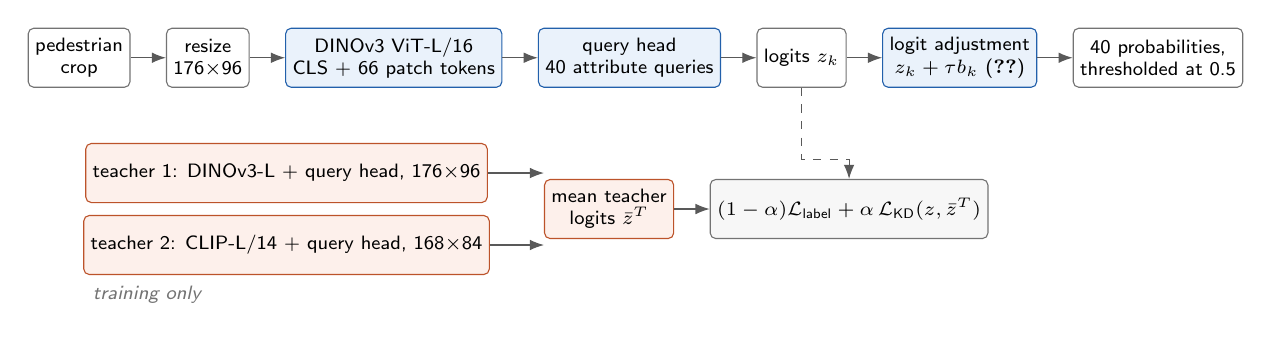
\begin{tikzpicture}[font=\sffamily\scriptsize, node distance=3.5mm and 4.5mm,
  box/.style={draw=black!55, rounded corners=2pt, fill=white, align=center, minimum height=7.5mm, inner sep=2.5pt},
  hl/.style={box, fill=acc!10, draw=acc!80!black}, tc/.style={box, fill=org!10, draw=org!80!black},
  arr/.style={-{Latex[length=1.8mm]}, black!65}]
\node[box] (img) {pedestrian\\ crop};
\node[box, right=of img] (rs) {resize\\ 176$\times$96};
\node[hl, right=of rs] (bb) {DINOv3 ViT-L/16\\ CLS + 66 patch tokens};
\node[hl, right=of bb] (qh) {query head\\ 40 attribute queries};
\node[box, right=of qh] (lg) {logits $z_k$};
\node[hl, right=of lg] (th) {logit adjustment\\ $z_k+\tau b_k$ (\cref{sec:rule})};
\node[box, right=of th] (pr) {40 probabilities,\\ thresholded at 0.5};
\draw[arr] (img)--(rs); \draw[arr] (rs)--(bb); \draw[arr] (bb)--(qh); \draw[arr] (qh)--(lg); \draw[arr] (lg)--(th); \draw[arr] (th)--(pr);
\node[tc, below=7mm of rs, xshift=10mm] (t1) {teacher 1: DINOv3-L + query head, 176$\times$96};
\node[tc, below=1.5mm of t1] (t2) {teacher 2: CLIP-L/14 + query head, 168$\times$84};
\node[tc, right=7mm of $(t1.east)!0.5!(t2.east)$] (avg) {mean teacher\\ logits $\bar z^{T}$};
\node[box, right=of avg, fill=black!3] (loss) {$(1-\alpha)\mathcal{L}_{\text{label}}+\alpha\,\mathcal{L}_{\text{KD}}(z,\bar z^{T})$};
\draw[arr] (t1.east)--(avg.west |- t1.east); \draw[arr] (t2.east)--(avg.west |- t2.east); \draw[arr] (avg)--(loss);
\draw[arr, dashed] (lg.south) |- ($(loss.north)+(0,2.5mm)$) -- (loss.north);
\node[font=\sffamily\scriptsize\itshape, text=black!55, anchor=west] at ($(t2.south west)+(0,-2.5mm)$) {training only};
\end{tikzpicture}
\caption{Submitted system. Top: the deployed model. Bottom: distillation, used only during training. Each teacher receives the same augmented batch, resized and re-normalized for its own input.}
\label{fig:pipeline}
\end{figure*}

\paragraph{Leave-one-dataset-out protocol.} In-domain validation was useless for design decisions (0.885 there versus 0.777 on the test). We therefore train on the training splits of two datasets and evaluate on the validation split of the third. PETA is held out in most experiments; Market1501 and PA100k serve as checks. We report three versions of Avg that differ only in the decision rule: \emph{raw} (logits as they are), \emph{offsets} (per-attribute offsets fitted on the seen datasets' validation data and scaled by $s=0.6$, our earlier rule), and $\tau$ (the rule of \cref{sec:rule} with $\tau=0.42$). Mean AUC measures ranking independently of any threshold. Protocol runs are shorter (3--10 epochs, two datasets) than submitted runs (10 epochs on training and validation data of all three).

\paragraph{Noise model.} Three pairs of runs in our logs differ only in the random seed (\cref{tab:noise}). They show that thresholded scores are noisy: one pair differs by 0.46\pts\ under fitted offsets. We pool the pairs into a standard deviation per metric and treat differences below about twice that value as ties. For offsets this means 0.4\pts, which is larger than many effects reported in the PAR literature. The head and resolution sweeps (\cref{tab:sweep,tab:res}) come from an earlier batch of runs without saved logits; its one replicate pair differs by 0.05\pts\ (offsets), 0.16\pts\ (raw) and 0.33\pts\ (AUC). We compare numbers only within a batch.

\begin{table}[t]
\centering\small
\setlength{\tabcolsep}{3pt}
\resizebox{\columnwidth}{!}{%
\begin{tabular}{@{}lcccc@{}}
\toprule
Seed pair (PETA held out) & raw & offsets & $\tau$ & AUC \\
\midrule
ViT-L query, 3 ep & 79.71 / 79.78 & 80.26 / 80.72 & 80.78 / 80.80 & 91.26 / 91.28 \\
ViT-B query, 5 ep & 78.78 / 78.83 & 79.46 / 79.31 & 79.48 / 79.40 & 90.19 / 90.00 \\
ViT-B linear, 5 ep & 78.01 / 77.29 & 79.03 / 79.02 & 79.05 / 79.14 & 90.35 / 90.41 \\
\midrule
pooled SD (pts) & 0.30 & 0.20 & 0.05 & 0.08 \\
\bottomrule
\end{tabular}}
\caption{Run-to-run noise from seed-only pairs (values $\times100$). The $\tau$ rule is the least noisy readout of the same logits.}
\label{tab:noise}
\end{table}

%=====================================================================
\section{Where the Cross-Domain Loss Comes From}
\label{sec:gap}

To separate threshold placement from ranking, we fit per-attribute offsets on the \emph{held-out} labels themselves. This oracle cannot be used at test time, but its gain over source-fitted offsets bounds what any threshold rule could recover; whatever remains is a ranking problem. \Cref{tab:gap} applies it to four models on all three held-out datasets.

\begin{table}[t]
\centering\small
\setlength{\tabcolsep}{2.8pt}
\begin{tabular}{@{}lcccc@{}}
\toprule
Held out & PETA & Market & PA100k & PETA \\
Model & ViT-B & ViT-B & ViT-B & ViT-L \\
\midrule
Avg, raw & 78.78 & 84.21 & 76.77 & 79.68 \\
Avg, source offsets & 79.46 & 84.64 & 79.75 & 80.33 \\
Avg, oracle offsets & 81.65 & 86.90 & 82.10 & 82.50 \\
\textbf{threshold gap} & \textbf{2.19} & \textbf{2.26} & \textbf{2.35} & \textbf{2.17} \\
\midrule
$\Delta$BA upper colors (12) & +3.7 & +2.6 & +7.4 & +4.0 \\
$\Delta$BA lower colors (12) & +5.3 & +6.8 & +6.1 & +4.3 \\
$\Delta$BA age (3) & $-$2.7 & +6.7 & +6.3 & $-$3.0 \\
$\Delta$BA hair (3) & $-$2.9 & +4.2 & $-$0.1 & $-$1.9 \\
$\Delta$BA other (10) & +0.8 & +2.2 & +2.4 & +1.8 \\
\bottomrule
\end{tabular}
\caption{Threshold component of the domain gap (query head). The oracle fits offsets on the held-out labels; $\Delta$BA is its gain in balanced accuracy per attribute group. Colors gain on every dataset; other groups vary.}
\label{tab:gap}
\end{table}

The threshold gap is remarkably constant: 2.2--2.4\pts\ on every held-out dataset, for both encoder sizes. It is also larger than every design change in \cref{sec:ranking}, so a reader who only tunes the network leaves this part untouched. Clothing colors gain on all four rows, while age and hair gain on some datasets and lose on others because the oracle maximizes Avg rather than mA.

Why do color thresholds fail to transfer? A plausible cause is that color names are applied differently across datasets. PETA labels 11.7\% of upper garments with two colors, whereas PA100k and Market1501 almost never do, so a ``grey'' decision learned on one dataset means something different on another. White-balance augmentation, which targets a camera color cast, did not improve held-out Avg (\cref{app:sweep}). We cannot confirm the labeling explanation without target labels, but it implies a clear design consequence: thresholds tuned on any source dataset partly encode that dataset's conventions. The protocol should therefore be trusted most for changes that raise AUC, and least for changes that only move thresholded Avg.

%=====================================================================
\section{Ranking: the Encoder Is the Lever}
\label{sec:ranking}

\paragraph{The head, loss and augmentation do not change ranking.} We ran 25 variants of the head, the loss and the augmentation on a fixed ViT-B encoder (\cref{tab:sweep}, all listed in \cref{app:sweep}). None improves Avg under offsets by more than 0.08\pts, inside the 0.4\pts\ noise band, and several lose: a CNN head loses 0.67\pts, a four-layer decoder 0.49\pts, and logit adjustment during training collapses by 12.2\pts, consistent with its shift adding to the DeepMAR and offset shifts. Their AUC stays within 0.898--0.908. A head can only re-weight the features it receives; on an unseen domain, these results indicate that the features, not their weighting, limit ranking.

\begin{table}[t]
\centering\small
\setlength{\tabcolsep}{4pt}
\resizebox{\columnwidth}{!}{%
\begin{tabular}{@{}lcccc@{}}
\toprule
Group (ViT-B, PETA held out) & \# & best $\Delta$ & worst $\Delta$ & AUC range \\
\midrule
Head architecture & 13 & +0.08 & $-$0.67 & 0.898--0.907 \\
Loss and training & 8 & +0.06 & $-$12.21 & 0.900--0.905 \\
Data and augmentation & 4 & $-$0.17 & $-$0.37 & 0.900--0.905 \\
\bottomrule
\end{tabular}}
\caption{Avg change (offsets, pts) relative to the query head on ViT-B (0.7958, mean of two runs). No variant leaves the noise band upwards.}
\label{tab:sweep}
\end{table}

\paragraph{The query head places thresholds, it does not rank better.} The query head is the one head change we kept, and the decomposition explains why its gain should be read with care. On both encoders it raises thresholded Avg but slightly lowers AUC (\cref{tab:head}). Its benefit is therefore a better-placed 0.5 threshold on the source domains, not better ranking, and by \cref{sec:gap} such benefits transfer least. The hidden test agrees in sign: ViT-B with the linear head scored 0.7775 and with the query head 0.7750, a difference within the test-set noise discussed in \cref{sec:test}.

\begin{table}[t]
\centering\small
\setlength{\tabcolsep}{3.5pt}
\resizebox{\columnwidth}{!}{%
\begin{tabular}{@{}llcccc@{}}
\toprule
Encoder & Head & raw & offsets & $\tau$ & AUC \\
\midrule
ViT-L 176 & linear & 78.04 & 79.23 & 79.70 & 91.18 \\
ViT-L 176 & query & 79.68 & 80.33 & 80.65 & 90.71 \\
ViT-B 256 & linear (2 seeds) & 77.65 & 79.03 & 79.10 & 90.38 \\
ViT-B 256 & query (2 seeds) & 78.81 & 79.39 & 79.44 & 90.10 \\
\bottomrule
\end{tabular}}
\caption{Linear versus query head (PETA held out, 5 epochs). The query head wins every thresholded readout and loses on AUC.}
\label{tab:head}
\end{table}

\paragraph{Encoder family and size.} Among L-size encoders fine-tuned with the same recipe (\cref{app:encoders}), the larger MetaCLIP2-H and DINOv3-L have the highest AUC (91.4 and 91.3), while CLIP-L has the best thresholded Avg. EVA02-L, despite its size, is the weakest. Moving from ViT-B to ViT-L raises AUC by 0.6--0.8\pts\ for the same head (\cref{tab:head}), the first architectural change in this study that moves ranking beyond noise.

\paragraph{Resolution, not depth, is the cheap dimension.} The time budget forces a smaller ViT-L, and the question is what to shrink. \Cref{tab:res} compares options. Reducing the input to $176\times96$ (66 tokens) keeps ViT-L ahead of ViT-B on every readout, but at $160\times80$ (50 tokens) it falls behind ViT-B, so there is a floor below which the larger encoder loses its advantage. Keeping only the first 18 of 24 blocks at $224\times112$ costs 1.3\pts\ of raw Avg and 0.4\pts\ of AUC against the full-depth model at the same resolution. Larger inputs than 176 raise the offsets readout (up to +0.66\pts\ at $224\times112$) without raising raw Avg or AUC, so by \cref{sec:gap} we did not pay their extra cost.

\begin{table}[t]
\centering\small
\setlength{\tabcolsep}{3pt}
\begin{tabular}{@{}lccccc@{}}
\toprule
Encoder & Input & Tokens & raw & offsets & AUC \\
\midrule
ViT-B & 256$\times$128 & 128 & 78.7 & 79.6 & 90.2 \\
ViT-L & 160$\times$80 & 50 & 77.9 & 78.9 & 89.6 \\
ViT-L & 176$\times$96 & 66 & 79.6 & 80.1 & 91.0 \\
ViT-L & 192$\times$96 & 72 & 79.4 & 80.1 & 90.8 \\
ViT-L & 224$\times$112 & 98 & 79.7 & 80.7 & 91.0 \\
\midrule
ViT-L, 24 blocks$^\dagger$ & 224$\times$112 & 98 & 80.1 & 80.6 & 91.7 \\
ViT-L, 18 blocks$^\dagger$ & 224$\times$112 & 98 & 78.8 & 79.4 & 91.3 \\
\bottomrule
\end{tabular}
\caption{Shrinking ViT-L (query head, PETA held out). Upper block: earlier batch, 5 epochs (ViT-B: mean of the replicate pair); $^\dagger$lower block: 3 epochs. Resolution above 176 helps only the offsets readout; cutting depth hurts all readouts.}
\label{tab:res}
\end{table}

%=====================================================================
\section{Ranking: Teachers and Distillation}
\label{sec:teachers}

\paragraph{What makes a good partner for DINOv3.} Larger, higher-resolution and differently pretrained models rank better than the deployable ViT-L, so we use them as teachers. Ensemble theory~\cite{krogh} says a partner helps through its own accuracy and through how differently it errs. To weigh the two, we fine-tuned nine other foundation models and averaged each one's logits with DINOv3-L's (\cref{fig:pairing}). Partner accuracy predicts the pair's gain almost perfectly (Spearman 0.93 across the nine), while logit correlation has a small negative partial effect once accuracy is accounted for ($-$0.15\pts\ per standard deviation in a joint linear fit). A second DINOv3-L at higher resolution is as accurate as CLIP-L but much more correlated (0.96), and the same fit predicts its smaller gain exactly. In practice this means choosing the most accurate partner of a different pretraining family: CLIP-L, then MetaCLIP2-H~\cite{metaclip2}. Adding both to DINOv3-L is within noise of adding CLIP-L alone (\cref{app:encoders}).

\begin{figure}[t]
\centering
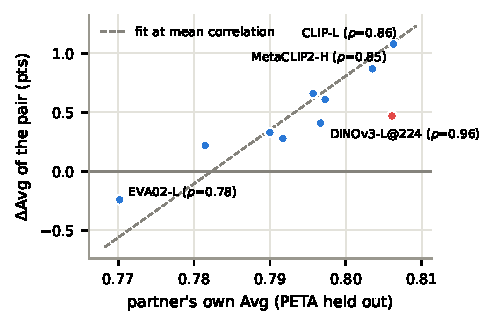
\includegraphics[width=\linewidth]{pairing.pdf}
\caption{Gain of averaging DINOv3-L with each partner, against the partner's own Avg (PETA held out, offsets). $\rho$ is the partner's logit correlation with DINOv3-L. Unlabeled points: PE-Core-L, SigLIP2-So400m, ConvNeXt-L, MetaCLIP2-L, SigLIP2-L, AIMv2-L.}
\label{fig:pairing}
\end{figure}

\paragraph{Distillation.} The student minimizes $(1-\alpha)\mathcal{L}_{\text{label}}+\alpha\,\mathrm{BCE}(\sigma(z),\sigma(\bar z^T))$ with $\alpha=0.8$, where $\bar z^T$ is the mean logit of the two teachers. Each teacher is fine-tuned for three epochs and sees the student's augmented batch at its own resolution and normalization, so that it stays in the regime it was trained for.

\begin{table}[t]
\centering\small
\setlength{\tabcolsep}{3.2pt}
\resizebox{\columnwidth}{!}{%
\begin{tabular}{@{}lccccc@{}}
\toprule
ViT-L 176 student & epochs & raw & $\tau$ & AUC & mADM \\
\midrule
label only & 3 & 79.75 & 80.79 & 91.27 & 65.15 \\
label only & 5 & 79.68 & 80.65 & 90.71 & 64.96 \\
distilled (DINOv3-L + CLIP-L) & 3 & 79.48 & 80.76 & 91.84 & 65.55 \\
distilled & 6 & 79.82 & 80.98 & 92.05 & 66.35 \\
distilled & 10 & 79.80 & 81.18 & 92.22 & 66.81 \\
distilled + DINOv3-L@224 & 6 & 79.68 & 80.77 & 91.94 & 65.90 \\
\bottomrule
\end{tabular}}
\caption{Distillation on PETA held out (values $\times100$; label-only 3-epoch row is the mean of the seed pair). mADM is the Track~2 retrieval metric on the same logits.}
\label{tab:kd}
\end{table}

\Cref{tab:kd} separates two effects. At equal length (3 epochs), distillation raises AUC by 0.6\pts\ but leaves raw and $\tau$ Avg within noise. Its larger effect is on training length: the label-only model gets worse from 3 to 5 epochs (AUC $-$0.6\pts), consistent with fitting the source datasets, while the distilled model keeps improving up to 10 epochs (AUC +0.4\pts, $\tau$ Avg +0.4\pts\ over its 3-epoch value). The teachers' soft targets thus act as a regularizer that makes longer training safe. A third, DINOv3-like teacher slightly hurts, consistent with the pairing result. Adding distillation targets on the cells that lack labels (Market1501 omits some attributes) had no measurable effect in a group-cross-entropy model ($\tau$ 80.57 vs 80.55), so we do not claim that teachers help by filling missing labels. At ten epochs the student slightly exceeds the AUC of the two-teacher ensemble (92.2 vs 92.0, \cref{app:encoders}) and recovers about half of its $\tau$ gain (+0.4 of +0.7\pts). Its improvement shows most in AUC and in the retrieval metric, which uses the whole probability vector.

%=====================================================================
\section{Thresholds: One Coefficient Instead of Forty}
\label{sec:rule}

\Cref{sec:gap} showed that thresholds fitted on source data absorb source conventions, and \cref{tab:noise} shows they also amplify training noise. We therefore look for a decision rule that has few free parameters and whose target does not depend on the unknown test domain.

\paragraph{Derivation.} The mA half of the metric is balanced accuracy, whose Bayes-optimal decision is the one made under a balanced prior, whatever the target prior is. If the model is calibrated under the training prior $\pi_k$, moving to a balanced prior adds $\log\frac{1-\pi_k}{\pi_k}$ to the logit~\cite{saerens,logitadj}. DeepMAR weighting has already moved the optimum of the training loss by $\log(w_k^+/w_k^-)=1-2\pi_k$ in the same direction, so the remaining correction is
\begin{equation}
b_k=\log\frac{1-\pi_k}{\pi_k}-(1-2\pi_k),\qquad z_k\leftarrow z_k+\tau\,b_k .
\label{eq:rule}
\end{equation}
Instance F1 prefers unbalanced decisions, so a shared $\tau\in[0,1]$ interpolates between the weighted-loss decision ($\tau=0$) and the mA-optimal one ($\tau=1$). For ``old'' ($\pi\approx0.03$) $b_k\approx2.5$; for ``trousers'' ($\pi\approx0.8$) $b_k\approx-0.8$. The derivation ignores label smoothing and the distillation term, both of which also shift the loss optimum, and it assumes calibration under $\pi_k$.

\paragraph{Stability.} Because the rule has one parameter and no fitted per-attribute offsets, it should be insensitive to training noise. \Cref{tab:noise} confirms this: across seed pairs, the $\tau$ readout varies with a pooled SD of 0.05\pts, against 0.20 for offsets and 0.30 for raw logits. On the worst pair, offsets differ by 0.46\pts\ while $\tau$ differs by 0.02.

\paragraph{Transfer.} We set $\tau=0.42$ on the PETA-held-out runs, where it beats the best offset scale ($s=0.75$) in 36 of 41 runs; this is in-sample. Two out-of-sample tests give a mixed picture (\cref{fig:thr}). Selecting both $s$ and $\tau$ on the seven Market1501- and PA100k-held-out runs ($s=1.0$, $\tau=0.3$) and testing on PETA, the rule wins in 35 of 41 runs (+0.26\pts\ on average). Selecting on PETA ($s=0.75$, $\tau=0.42$) and testing on the other datasets, it wins all five Market1501 runs by 0.2--0.6\pts\ but loses both PA100k runs, by 0.55\pts\ for the query head and by 9.7\pts\ for the linear head. The PA100k fold is the case the derivation excludes: holding out PA100k removes 81\% of the training data, the remaining priors come from 18.7k images, and the linear model on this fold is badly calibrated (held-out NLL 11.2 nats per image against 7.6 for the query head). The rule should therefore be used only when the training prior is estimated from representative data, as in the submitted system, which trains on all three datasets.

\begin{figure*}[t]
\centering
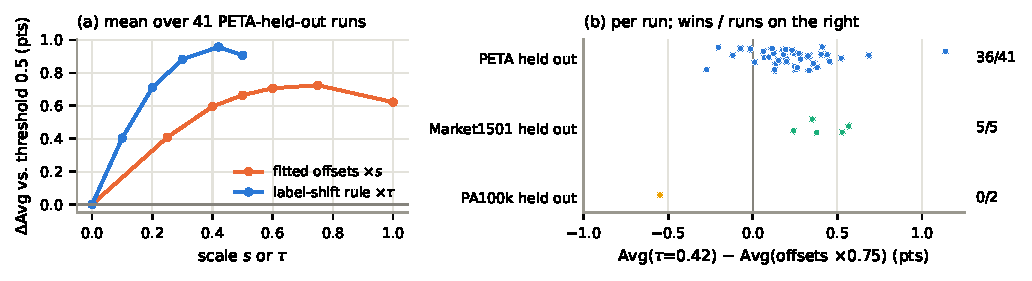
\includegraphics[width=\linewidth]{thresholds.pdf}
\caption{Label-shift rule versus source-fitted offsets. (a) Mean gain over the 0.5 threshold on the 41 PETA-held-out runs; $\tau=0.42$ and $s=0.75$ were read from these curves. (b) Difference per run between the two rules at those settings. The Market1501 and PA100k runs are out-of-sample; the PA100k linear-head run ($-$9.7\pts) lies outside the axis.}
\label{fig:thr}
\end{figure*}

%=====================================================================
\section{What the Query Head Looks At}
\label{sec:xai}

The query head was motivated by letting each attribute read its own image region (\cref{sec:setting}). To check whether it does so on an unseen domain, we take the query-head model trained without PETA (ViT-B, $256\times128$) and inspect PETA validation images it has never seen. For each of six attributes we select the most confident correct positive and the most confident error under the $\tau$ rule. \Cref{fig:xai} shows, for each case, the image, the cross-attention of that attribute's query over the $16\times8$ patch tokens (averaged over the 8 heads; the share left on the CLS token is at most 1\% in all twelve cases), and Integrated Gradients~\cite{ig} of the attribute's logit with a mean-colour baseline (24 steps, pooled to $8\times8$ pixels; red raises the logit, blue lowers it).

\begin{figure}[t]
\centering
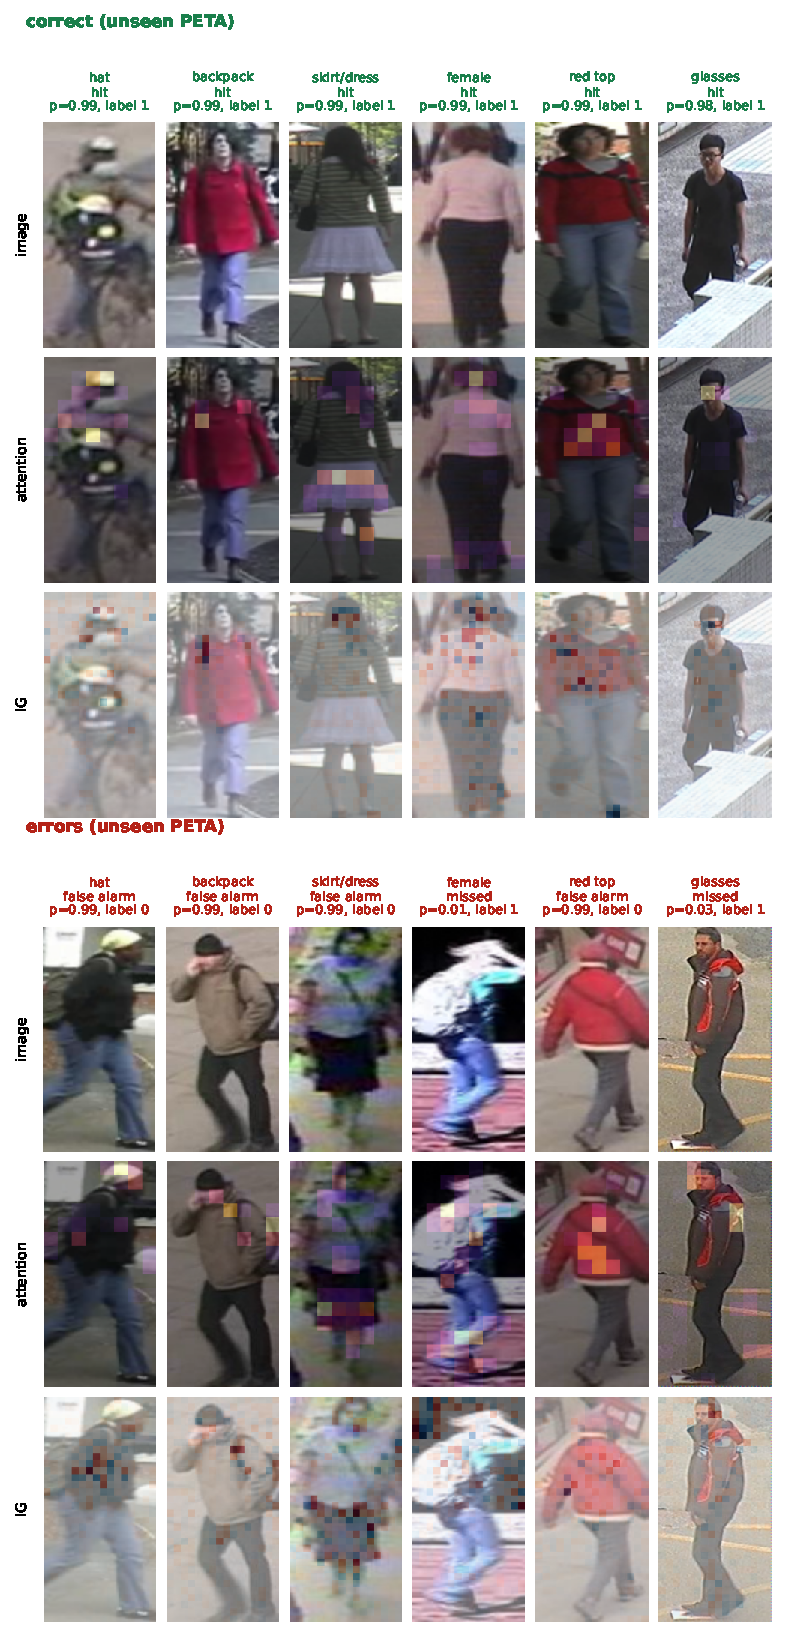
\includegraphics[width=\linewidth]{xai_cases.pdf}
\caption{Correct cases (top) and errors (bottom) of a model that never saw PETA, on PETA validation images. Rows: image with the attribute, decision, probability and label; attention of the attribute's query; Integrated Gradients. The errors are the most confident ones for each attribute.}
\label{fig:xai}
\end{figure}

In all six correct cases the attention falls on the region the attribute describes: the head for hat and glasses, the shoulder strap for backpack, the lower body for skirt and the torso for the red top; for female it covers the head and hair. The errors are more informative. In three of them the image, by visual inspection, contradicts the label: a person in a light cap labelled without a hat, a red jacket labelled as not a red top, and a strap across the shoulder labelled as no backpack. Attention sits on the right region in each, so these look like labelling conventions or label noise rather than failures of the model, consistent with the labelling-convention explanation of \cref{sec:gap}. The skirt false alarm is a heavily blurred image with a dark lower garment. The two misses are failures of perception: for female, a blurred back view, attention spreads over the body and onto the ground; for glasses, the face covers only a few patches. Integrated Gradients is much noisier than attention at this resolution and mostly marks the same regions. These are twelve selected cases; they show what the head does, not how often each kind of error occurs.

\paragraph{Occlusion.} Attention shows where a query reads, not what the decision depends on. We therefore hide regions and measure the effect on all 6{,}963 unseen PETA validation images. The crop is split into three horizontal bands (head: the top 20\% of the height; upper body: 20--55\%; lower body: 55--100\%), and each band is either filled with the mean colour or kept alone. \Cref{fig:occ} reports the change in held-out AUC per attribute group. Every group depends mainly on the band it describes. Masking the head lowers AUC by 0.25 for hat, 0.21 for glasses and 0.16 for hair length; masking the upper body lowers it by 0.22 for sleeve length and 0.24 for backpack and bag; masking the lower body lowers it by 0.22 for lower length and 0.16 for lower colour. Keeping only that band costs far less: 0.04 for hat and 0.02 for lower colour. Age relies on the head, which alone gives the full-image AUC (0.754 against 0.751). Gender is the exception. Masking any single band costs at most 0.05, and no band alone comes close to the full image (0.78--0.85 against 0.95), so the model combines evidence from the whole body. A sliding $32\times32$ occlusion on the twelve cases of \cref{fig:xai} agrees with the attention maps (\cref{fig:occmaps}): the logit falls most when the region named by the attribute is hidden, such as the head for hat and glasses, the torso for the red top and the lower body for the skirt, and this holds for the errors that look like label conventions as well.

\begin{figure}[t]
\centering
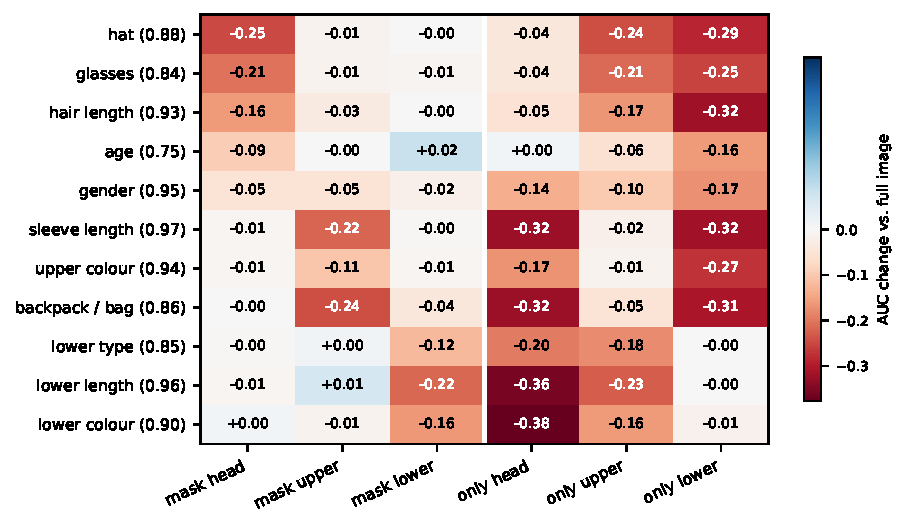
\includegraphics[width=\linewidth]{occlusion_auc.pdf}
\caption{Change in held-out AUC when one horizontal band is masked (left three columns) or kept alone (right three), on all PETA validation images, for a model that never saw PETA. The full-image AUC is given after each group name.}
\label{fig:occ}
\end{figure}

\begin{figure}[t]
\centering
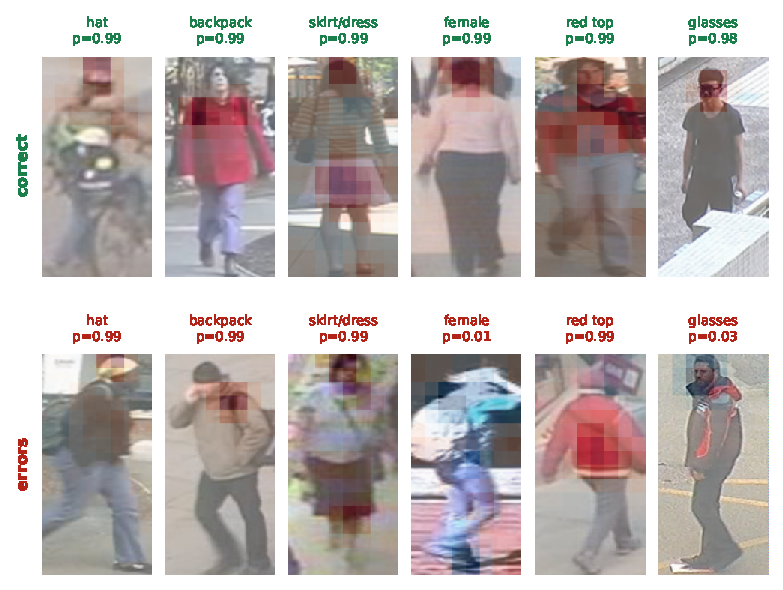
\includegraphics[width=\linewidth]{occlusion_maps.pdf}
\caption{Sliding occlusion on the cases of \cref{fig:xai}: drop of the attribute's logit when a $32\times32$ mean-colour square covers each position. Red: the square hid evidence for the attribute; blue: evidence against it.}
\label{fig:occmaps}
\end{figure}

%=====================================================================
\section{Hidden-Test Results}
\label{sec:test}

\Cref{tab:main} lists the submissions with the factors each one changed. Only one pair of submissions isolates training noise on the test set: v9 and v10 share the recipe and differ only in adding validation data, and they differ by 0.19\pts. Steps smaller than this cannot be attributed. Against this yardstick, moving from ViT-B to ViT-L with the same head (v8 to v9, +1.07\pts) is clearly real, distillation together with a longer schedule (+0.58\pts) is likely real, and the threshold rule (+0.16\pts) is consistent with the protocol but not established by the test. The organizers' 2027 baseline score was not available to us, so we cannot report the margin over it.

\begin{table}[t]
\centering\small
\setlength{\tabcolsep}{3pt}
\resizebox{\columnwidth}{!}{%
\begin{tabular}{@{}llcc@{}}
\toprule
& Changed factors & $\tau$ / offsets (LODO) & Test \\
\midrule
v4b & ViT-B, linear head, offsets & 79.04 & 77.75 \\
v8 & query head & 79.58 & 77.50 \\
v9 & ViT-L 176 & 80.05 & 78.57 \\
v10 & + validation data & -- & 78.38 \\
v12 & + distillation, 10 epochs & 80.57 & 78.96 \\
v13 & + label-shift rule & 81.18 & \textbf{79.12} \\
\midrule
v18 & ViT-B student, function matching, rule & 80.24$^\dagger$ & 78.23 \\
\bottomrule
\end{tabular}}
\caption{Hidden-test submissions (values $\times100$). LODO is the PETA-held-out score of the same recipe and rule; LODO values for v4b--v9 come from the earlier batch; $^\dagger$10-epoch proxy of a 20-epoch recipe. The v9/v10 difference (0.19\pts) is the only test-set replicate.}
\label{tab:main}
\end{table}

%=====================================================================
\section{Discussion}

\paragraph{What transfers.} The analyses point the same way. Ranking, measured by AUC, responds to the encoder and to what the encoder is taught, and these gains survive on the hidden test. Threshold placement fitted on source data costs a stable 2.2\pts, does not transfer, and is noisy; a rule with one coefficient and a domain-independent target reduces the noise, though it inherits the assumptions of its derivation. For practitioners, the decomposition suggests a simple check before investing in a component: if a change improves thresholded accuracy without improving AUC, expect it to transfer poorly.

\paragraph{Limitations.} Noise estimates rest on three seed pairs. Most experiments hold out PETA. Protocol runs are shorter than submitted runs. The labeling explanation for color thresholds is plausible but untested, and a single-teacher student was not trained, so the contribution of each teacher to the student is unknown.

\paragraph{Broader impact.} Attribute recognition on surveillance video, including age and gender, can support tracking of individuals. We report technical findings only and do not release models trained on surveillance data.

\section{Conclusion}

On unseen cameras, pedestrian attribute recognition loses about 2.2 points to threshold placement that source data cannot fix, and the rest is a ranking problem that only the encoder and its training signal address. Designing for this split led us to a reduced-resolution DINOv3 ViT-L distilled from complementary teachers, and to a one-coefficient logit adjustment that is stable across runs but must be used with representative priors.

{\small
\begin{thebibliography}{99}\setlength{\itemsep}{0pt}
\bibitem{upar} A.~Specker, M.~Cormier, J.~Beyerer. UPAR: Unified pedestrian attribute recognition and person retrieval. In \textit{WACV}, 2023.
\bibitem{upar23} M.~Cormier \etal. UPAR challenge: Pedestrian attribute recognition and attribute-based person retrieval -- dataset, design, and results. In \textit{WACV Workshops}, 2023.
\bibitem{upar24} M.~Cormier \etal. UPAR challenge 2024: Pedestrian attribute recognition and attribute-based person retrieval -- dataset, design, and results. In \textit{WACV Workshops}, 2024.
\bibitem{peta} Y.~Deng, P.~Luo, C.~C.~Loy, X.~Tang. Pedestrian attribute recognition at far distance. In \textit{ACM MM}, 2014.
\bibitem{pa100k} X.~Liu \etal. HydraPlus-Net: Attentive deep features for pedestrian analysis. In \textit{ICCV}, 2017.
\bibitem{market} L.~Zheng \etal. Scalable person re-identification: A benchmark. In \textit{ICCV}, 2015.
\bibitem{marketattr} Y.~Lin \etal. Improving person re-identification by attribute and identity learning. \textit{Pattern Recognition}, 2019.
\bibitem{deepmar} D.~Li, X.~Chen, K.~Huang. Multi-attribute learning for pedestrian attribute recognition in surveillance scenarios. In \textit{ACPR}, 2015.
\bibitem{parsurvey} X.~Wang \etal. Pedestrian attribute recognition: A survey. \textit{Pattern Recognition}, 2022.
\bibitem{rethinkpar} J.~Jia, H.~Huang, X.~Chen, K.~Huang. Rethinking of pedestrian attribute recognition: A reliable evaluation under zero-shot pedestrian identity setting. \textit{arXiv:2107.03576}, 2021.
\bibitem{q2l} S.~Liu \etal. Query2Label: A simple transformer way to multi-label classification. \textit{arXiv:2107.10834}, 2021.
\bibitem{mldecoder} T.~Ridnik \etal. ML-Decoder: Scalable and versatile classification head. In \textit{WACV}, 2023.
\bibitem{domainbed} I.~Gulrajani, D.~Lopez-Paz. In search of lost domain generalization. In \textit{ICLR}, 2021.
\bibitem{krogh} A.~Krogh, J.~Vedelsby. Neural network ensembles, cross validation, and active learning. In \textit{NeurIPS}, 1995.
\bibitem{kuncheva} L.~I.~Kuncheva, C.~J.~Whitaker. Measures of diversity in classifier ensembles and their relationship with the ensemble accuracy. \textit{Machine Learning}, 2003.
\bibitem{hinton} G.~Hinton, O.~Vinyals, J.~Dean. Distilling the knowledge in a neural network. \textit{arXiv:1503.02531}, 2015.
\bibitem{radio} M.~Ranzinger, G.~Heinrich, J.~Kautz, P.~Molchanov. AM-RADIO: Agglomerative vision foundation model -- reduce all domains into one. In \textit{CVPR}, 2024.
\bibitem{patient} L.~Beyer \etal. Knowledge distillation: A good teacher is patient and consistent. In \textit{CVPR}, 2022.
\bibitem{saerens} M.~Saerens, P.~Latinne, C.~Decaestecker. Adjusting the outputs of a classifier to new a priori probabilities: A simple procedure. \textit{Neural Computation}, 2002.
\bibitem{lipton} Z.~C.~Lipton, Y.-X.~Wang, A.~Smola. Detecting and correcting for label shift with black box predictors. In \textit{ICML}, 2018.
\bibitem{logitadj} A.~K.~Menon \etal. Long-tail learning via logit adjustment. In \textit{ICLR}, 2021.
\bibitem{dinov3} O.~Sim\'eoni \etal. DINOv3. \textit{arXiv:2508.10104}, 2025.
\bibitem{clip} A.~Radford \etal. Learning transferable visual models from natural language supervision. In \textit{ICML}, 2021.
\bibitem{metaclip2} Y.-S.~Chuang \etal. MetaCLIP 2: A worldwide scaling recipe. \textit{arXiv:2507.22062}, 2025.
\bibitem{siglip2} M.~Tschannen \etal. SigLIP 2: Multilingual vision-language encoders with improved semantic understanding, localization, and dense features. \textit{arXiv:2502.14786}, 2025.
\bibitem{pe} D.~Bolya \etal. Perception Encoder: The best visual embeddings are not at the output of the network. \textit{arXiv:2504.13181}, 2025.
\bibitem{eva02} Y.~Fang \etal. EVA-02: A visual representation for neon genesis. \textit{arXiv:2303.11331}, 2023.
\bibitem{aimv2} E.~Fini \etal. Multimodal autoregressive pre-training of large vision encoders. \textit{arXiv:2411.14402}, 2024.
\bibitem{convnext} Z.~Liu \etal. A ConvNet for the 2020s. In \textit{CVPR}, 2022.
\bibitem{asl} T.~Ridnik \etal. Asymmetric loss for multi-label classification. In \textit{ICCV}, 2021.
\bibitem{lpft} A.~Kumar \etal. Fine-tuning can distort pretrained features and underperform out-of-distribution. In \textit{ICLR}, 2022.
\bibitem{mixstyle} K.~Zhou, Y.~Yang, Y.~Qiao, T.~Xiang. Domain generalization with MixStyle. In \textit{ICLR}, 2021.
\bibitem{csra} K.~Zhu, J.~Wu. Residual attention: A simple but effective method for multi-label recognition. In \textit{ICCV}, 2021.
\bibitem{mamba} A.~Gu, T.~Dao. Mamba: Linear-time sequence modeling with selective state spaces. \textit{arXiv:2312.00752}, 2023.
\bibitem{ig} M.~Sundararajan, A.~Taly, Q.~Yan. Axiomatic attribution for deep networks. In \textit{ICML}, 2017.
\bibitem{soup} M.~Wortsman \etal. Model soups: Averaging weights of multiple fine-tuned models improves accuracy without increasing inference time. In \textit{ICML}, 2022.
\end{thebibliography}
}

\clearpage
\appendix
\onecolumn
\section{Full design sweep}
\label{app:sweep}

Variants are grouped as in \cref{tab:sweep}; references: ASL~\cite{asl}, LP-FT~\cite{lpft}, MixStyle~\cite{mixstyle}, CSRA~\cite{csra}, Mamba~\cite{mamba}, logit adjustment~\cite{logitadj}. ``Group cross-entropy'' adds a softmax cross-entropy within mutually exclusive attribute groups. All runs: ViT-B 256$\times$128, PETA held out, 5 epochs, last checkpoint, offsets $\times0.6$, unless stated otherwise.

\begin{table}[h]
\centering\small
\begin{tabular}{@{}llcc|llcc@{}}
\toprule
Group & Variant & Avg & AUC & Group & Variant & Avg & AUC \\
\midrule
Baseline & query head (run 1) & 0.7961 & 0.901 & Loss/training & MAE reconstruction decoder & 0.7944 & 0.900 \\
Baseline & query head (run 2) & 0.7956 & 0.904 & Loss/training & attribute reconstruction decoder & 0.7940 & 0.902 \\
Baseline & linear head & 0.7904 & 0.908 & Loss/training & LP-FT & 0.7937 & 0.903 \\
Head & body-part spatial prior & 0.7966 & 0.905 & Loss/training & 3 epochs instead of 5 & 0.7921 & 0.904 \\
Head & 2-layer query head & 0.7965 & 0.902 & Loss/training & group cross-entropy & 0.7919 & 0.905 \\
Head & group-sequential attention & 0.7964 & 0.907 & Loss/training & logit adjustment (training) & 0.6737 & 0.902 \\
Head & foreground-token prior & 0.7961 & 0.901 & Data/aug. & white-balance augmentation & 0.7941 & 0.900 \\
Head & query + linear heads & 0.7951 & 0.904 & Data/aug. & strong augmentation & 0.7940 & 0.901 \\
Head & tokens of last 4 blocks & 0.7946 & 0.899 & Data/aug. & balanced dataset sampling & 0.7927 & 0.905 \\
Head & spatial + foreground prior & 0.7943 & 0.902 & Data/aug. & MixStyle & 0.7921 & 0.900 \\
Head & Mamba scan over attributes & 0.7930 & 0.898 & & & & \\
Head & MoE on tokens & 0.7921 & 0.900 & & & & \\
Head & 4-layer decoder + self-attention & 0.7909 & 0.904 & & & & \\
Head & CNN head (CSRA, T=3) & 0.7905 & 0.900 & & & & \\
Head & per-dataset classifiers & 0.7899 & 0.901 & & & & \\
Head & CNN head (CSRA) & 0.7891 & 0.905 & & & & \\
Loss/training & ASL & 0.7964 & 0.903 & & & & \\
Loss/training & noisy-label masking (1\%) & 0.7959 & 0.904 & & & & \\
\bottomrule
\end{tabular}
\caption{All 25 head, loss and augmentation variants and the three baseline runs.}
\end{table}

\section{Encoders and teacher ensembles}
\label{app:encoders}

\begin{table}[h]
\centering\small
\begin{tabular}{@{}lccccc|lccc@{}}
\toprule
Encoder (L size, 3 epochs) & input & raw & offsets & $\tau$ & AUC & Logit average with DINOv3-L & offsets & $\tau$ & AUC \\
\midrule
DINOv3-L/16 (2 seeds) & 176$\times$96 & 79.75 & 80.49 & 80.79 & 91.27 & DINOv3-L alone & 80.26 & 80.78 & 91.26 \\
DINOv3-L/16 & 224$\times$112 & 80.09 & 80.61 & 80.95 & 91.67 & + CLIP-L & 81.34 & 81.46 & 92.03 \\
CLIP-L/14~\cite{clip} & 168$\times$84 & 79.96 & 80.63 & 80.85 & 90.86 & + MetaCLIP2-H & 81.13 & 81.49 & 92.39 \\
MetaCLIP2-H/14~\cite{metaclip2} & 168$\times$84 & 79.59 & 80.35 & 80.59 & 91.36 & + CLIP-L + MetaCLIP2-H & 81.37 & 81.68 & 92.48 \\
SigLIP2-So400m~\cite{siglip2} & 168$\times$84 & 78.82 & 79.73 & 79.92 & 91.07 & + CLIP-L, per-attribute weights & 81.20 & 81.48 & 91.92 \\
ConvNeXt-L (DINOv3)~\cite{convnext} & 256$\times$128 & 78.98 & 79.67 & 79.80 & 90.81 & & & & \\
PE-Core-L~\cite{pe} & 168$\times$84 & 79.09 & 79.57 & 79.76 & 90.72 & & & & \\
SigLIP2-L & 176$\times$96 & 78.69 & 79.17 & 79.33 & 90.76 & & & & \\
MetaCLIP2-L & 168$\times$84 & 78.49 & 79.00 & 79.30 & 90.32 & & & & \\
AIMv2-L~\cite{aimv2} & 168$\times$84 & 77.79 & 78.15 & 78.00 & 90.01 & & & & \\
EVA02-L~\cite{eva02} & 168$\times$84 & 76.24 & 77.02 & 76.91 & 88.49 & & & & \\
\bottomrule
\end{tabular}
\caption{Left: L-size encoders fine-tuned with the same recipe (query head, 8 frozen blocks, PETA held out). Right: teacher ensembles (logit averages, PETA held out). Values $\times100$.}
\end{table}

\section{Negative results}
\label{app:neg}

\begin{itemize}
\item \textbf{Dynamic int8 quantization} of the encoder: ViT-L on PETA held out drops from 80.9 to 76.5 Avg; ViT-B on in-domain validation from 88.5 to 70.3 (all linear layers) or 80.9 (attention projections and first MLP layer only).
\item \textbf{Model soups}~\cite{soup}: heads trained from different seeds collapse when averaged (about 75 Avg); soups from one initialization match their ingredients but do not exceed them.
\item \textbf{Distilling ViT-L into ViT-B with labels as targets only} (no mixed inputs): +0.17\pts\ on the protocol, $-$0.58\pts\ on the hidden test.
\item \textbf{Teacher-agreement weighting} and \textbf{teacher logit standardization}: no change over plain averaging.
\end{itemize}

\section{Configuration of v13}

Student: DINOv3 ViT-L/16 at $176\times96$, query head (1 layer, 8 heads, MLP ratio 2, dropout 0.1), first 8 blocks frozen, AdamW with learning rate $5\cdot10^{-5}$ at the last block and layer decay 0.75, head learning rate $\times10$, weight decay 0.05, batch 64, cosine schedule with 0.5 epoch warm-up, EMA 0.9995, 10 epochs on training and validation data of the three datasets, datasets sampled $\propto N_d^{0.5}$. Augmentation: flip, pad-and-crop, random down-scaling, brightness and contrast jitter, no hue change. Teachers: DINOv3-L ($176\times96$) and CLIP-L/14 ($168\times84$), 3 epochs each. Distillation $\alpha=0.8$, temperature 1. Decision rule $\tau=0.42$ with $\pi_k$ from training and validation data clipped to $[10^{-3},1-10^{-3}]$.

\end{document}
